Bibika está jogando o famoso jogo Navalha Batal.
Para quem não conhece, o jogo é disputado entre duas pessoas e um tabuleiro comum, de tamanho $N \times N$, com algumas peças (que representam Bavios) de tamanhos $1 \times T$ e $T \times 1$ previamente inseridas, onde o valor de $T$ é inteiro positivo menor ou igual a $N$.
A sobreposição de peças não é possível!

Após a posição das peças iniciais ser revelada, cada jogador tem alguns minutos para analisar o tabuleiro e calcular (ou chutar) a quantidade de peças $1 \times T$, $T \times 1$ diferentes que ainda podem ser inseridas no tabuleiro.
Duas peças são diferentes se os espaços que elas ocupam no tabuleiro são diferentes.

Segue um exemplo de um tabuleiro $3 \times 3$ com as posições $\left\{(1,2), (2,3), (3,1), (3,2)\right\}$ previamente preenchidas.

\begin{figure}[h!]
\centering
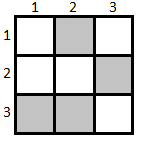
\includegraphics[scale=0.7]{\CWD/tab_inicial.png}
\end{figure}

Nesse caso ainda é possível inserir nas células vazias 7 peças diferentes, como ilustrado abaixo:

\begin{figure}[h!]
\centering
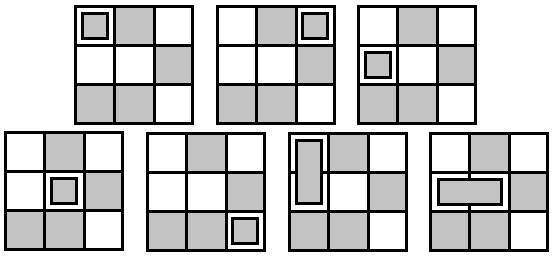
\includegraphics[scale=0.6]{\CWD/pecas.png}
\end{figure}

Após jogarem com um tabuleiro bem pequeno, Bibika gostaria de saber, dado um tabuleiro gigante e uma configuração inicial do tabuleiro, qual solução do jogo. Como é uma tarefa bastante complexa a olho nu, cabe a você ajudá-la!

\section*{Entrada}

A primeira linha contém dois inteiros $N$ e $Q$, sendo $N$ o tamanho do tabuleiro quadrado e $Q$ a quantidade de células distintas que estão previamente preenchidas.
As próximas $Q$ linhas possuem dois inteiros, $X_i$ e $Y_i$, indicando que a coordenada $X_i, Y_i$ do tabuleiro está preenchida.

\section*{Saída}

Exiba um único inteiro, a quantidade de bavios de tamanho $1 \times T$ ou $T \times 1$ que ainda são possíveis de serem colocados de forma que fiquem totalmente inseridos no tabuleiro e não exista sobreposição com outros bavios.

\section*{Restrições}

$1 \leq N \leq 10^6$
$0 \leq Q \leq 10^5$
$1 \leq X, Y \leq N$

\section*{Exemplos}
\exemplo
